\SourceLeaf{117}
alle aus dem Prinzip, dass die Produkte der voneinander abgewandten (bloß
eine gemeinsame Spitze oder, noch knapper gesagt, keine gemeinsame Seite
habenden) Dreiecke, in die ein Viereck durch seine Diagonalen zerlegt wird, gleich sind.

Die allgemeine baryzentrische Gleichung zwischen vier Punkten, z.\,B. $(A)$, $(B)$, $(C)$,
$(D)$ lautet
\[
\TriLetter{A}\,(A)+\TriLetter{B}\,(B)+\TriLetter{C}\,(C)+\TriLetter{D}\,(D)=0,
\]
wobei $\TriLetter{A}$ das Dreieck $BCD$, $\TriLetter{B}$ das Dreieck $CDA$
usw. (mit Rücksicht auf [das] Vorzeichen) bezeichnet. Ergänzt man in unserem
Fall die obigen Bezeichnungen durch
\[
\boldsymbol{A}^{*}=\alpha+\gamma+\delta+a+\lambda, \quad \text{usw.}
\]
\[
\boldsymbol{A}^{*}=\omega-\mathfrak{B}-\mathfrak{E}, \quad \text{usw.},
\]
so hat die Gleichung zwischen vier Punkten die Form
\[
\mathfrak{C}(A)+\boldsymbol{D}^{*}(C)=\boldsymbol{A}^{*}(B)+\mathfrak{B}(D),
\]
wobei $(A)$ den betreffenden Eckpunkt des äußeren Pentagons bezeichnet. Gleichwertig dazu ist
\[
\begin{gathered}\mathfrak{C}(A)+(\omega-\mathfrak{E}-\mathfrak{C})(C)\\=(\omega-\mathfrak{B}-\mathfrak{E})(B)+\mathfrak{B}(D)\\=(\omega-\mathfrak{E})(e),\end{gathered}
\]
wobei $(e)$ den betreffenden Punkt des inneren Pentagons bezeichnet.

\begin{center}\rule{3cm}{.4pt}\end{center}

\begin{center}\resizebox{7cm}{!}{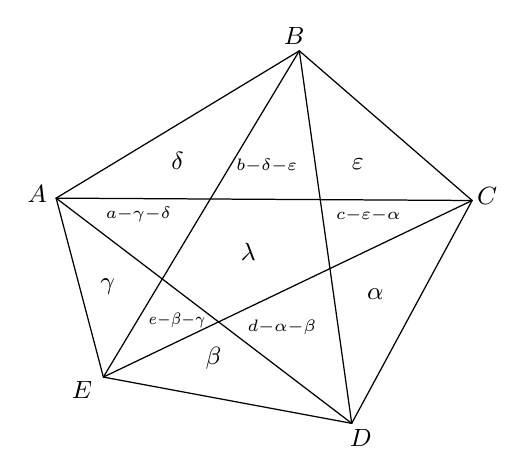
\begin{tikzpicture}[x=.006cm,y=-.006cm,line width=.45pt,line cap=round,line join=round,every node/.style={inner sep=0pt,font=\small}]
\coordinate (A) at (158,408);
\coordinate (B) at (673,96);
\coordinate (C) at (1039,413);
\coordinate (D) at (784,885);
\coordinate (E) at (258,787);
\draw (A) -- (B);
\draw (B) -- (C);
\draw (C) -- (D);
\draw (D) -- (E);
\draw (E) -- (A);
\draw (A) -- (C);
\draw (A) -- (D);
\draw (B) -- (E);
\draw (B) -- (D);
\draw (C) -- (E);
\node at (118,400) {$A$};
\node at (662,65) {$B$};
\node at (1071,403) {$C$};
\node at (803,916) {$D$};
\node at (213,814) {$E$};
\node at (415,330) {$\delta$};
\node at (604,339) {$\scriptstyle b-\delta-\varepsilon$};
\node at (797,337) {$\varepsilon$};
\node at (332,443) {$\scriptstyle a-\gamma-\delta$};
\node at (819,445) {$\scriptstyle c-\varepsilon-\alpha$};
\node at (565,522) {$\lambda$};
\node at (267,596) {$\gamma$};
\node at (414,666) {\scalebox{.86}[1]{$\scriptstyle e-\beta-\gamma$}};
\node at (491,747) {$\beta$};
\node at (636,681) {$\scriptstyle d-\alpha-\beta$};
\node at (834,612) {$\alpha$};
\end{tikzpicture}
}\end{center}

\[
\boldsymbol{A}c\varepsilon+\boldsymbol{C}c(b-\varepsilon)=\boldsymbol{B}b(c-\varepsilon)+\boldsymbol{D}b\varepsilon,
\]
\[
\boldsymbol{B}d\alpha+\boldsymbol{D}d(c-\alpha)=\boldsymbol{C}c(d-\alpha)+\boldsymbol{E}c\alpha,
\]
\[
\boldsymbol{C}e\beta+\boldsymbol{E}e(d-\beta)=\boldsymbol{D}d(e-\beta)+\boldsymbol{A}d\beta,
\]
\[
\boldsymbol{D}a\gamma+\boldsymbol{A}a(e-\gamma)=\boldsymbol{E}e(a-\gamma)+\boldsymbol{B}e\gamma,
\]
\[
\boldsymbol{E}b\delta+\boldsymbol{B}b(a-\delta)=\boldsymbol{A}a(b-\delta)+\boldsymbol{C}a\delta,
\]
